% ============================================================================
%  Institutional Representation ABM — Conference Poster
%
%  A0 portrait (841 mm x 1189 mm). Uses tikzposter. Render with:
%      tectonic poster.tex
%  or  pdflatex poster.tex
%
%  Content is a condensation of paper/main.tex — poster emphasises visuals,
%  headline findings, and takeaways. Two-column layout on a 25pt type scale.
% ============================================================================

\documentclass[25pt, a0paper, portrait, margin=10mm, innermargin=20mm,
               blockverticalspace=12mm, colspace=15mm, subcolspace=8mm]{tikzposter}

\usepackage[utf8]{inputenc}
\usepackage[T1]{fontenc}
\usepackage{lmodern}
\usepackage{booktabs}
\usepackage{amsmath}
\usepackage{graphicx}
\usepackage[scaled=0.95]{helvet}
\renewcommand{\familydefault}{\sfdefault}

\graphicspath{{../docs/figures/}}

% Clean academic colour scheme — blue accents, neutral background.
\definecolor{posterblue}{HTML}{1F4E79}
\definecolor{postergrey}{HTML}{E8EEF4}
\definecolor{posteraccent}{HTML}{D04A3A}

\definecolorstyle{PosterColors}{}{
    \colorlet{backgroundcolor}{white}
    \colorlet{framecolor}{posterblue}
    \colorlet{titlefgcolor}{white}
    \colorlet{titlebgcolor}{posterblue}
    \colorlet{blocktitlefgcolor}{white}
    \colorlet{blocktitlebgcolor}{posterblue}
    \colorlet{blockbodyfgcolor}{black}
    \colorlet{blockbodybgcolor}{postergrey}
    \colorlet{innerblocktitlefgcolor}{posterblue}
    \colorlet{innerblocktitlebgcolor}{white}
    \colorlet{innerblockbodyfgcolor}{black}
    \colorlet{innerblockbodybgcolor}{white}
    \colorlet{notefgcolor}{black}
    \colorlet{notebgcolor}{white}
    \colorlet{notefrcolor}{posterblue}
}

\usetheme{Default}
\usecolorstyle{PosterColors}
\useblockstyle{Default}

% Hide the default tikzposter footer.
\tikzposterlatexaffectionproofoff

% Custom title style so the long title fits without clipping and the
% subtitle/contact line is legible at poster distance.
\settitle{%
    \centering
    \vbox{%
        \color{titlefgcolor}
        \fontsize{70}{84}\selectfont\bfseries \@title \par
        \vspace{6mm}
        \fontsize{42}{50}\selectfont\normalfont
        A four-institution agent-based model of legislative passage \par
        \vspace{8mm}
        \fontsize{30}{36}\selectfont\normalfont \@author \par
        \vspace{5mm}
        \fontsize{22}{26}\selectfont\normalfont\ttfamily
        github.com/tofuadmiral/institutional-representation-abm
        \quad$\cdot$\quad
        institutional-representation-abm.streamlit.app
    }%
}

% ------------------------------------------------------------------ metadata
\title{Parliamentary Collapse Under Fragmentation}
\author{Fuad Ali}
\institute{}

\begin{document}
\maketitle[titletotopverticalspace=10mm, titletoblockverticalspace=15mm]

% ============================================================================
\begin{columns}

% ------------------------------------------------------ COLUMN 1 ------------
\column{0.33}

\block{The puzzle}{%
\large
Parliamentary systems pass more bills than presidential systems at
baseline, but collapse to near-zero passage when legislatures fragment.
Three competing mechanistic accounts exist in the literature:
coalition-formation failure, party discipline, and committee gatekeeping.

\medskip
\textbf{These three mechanisms operate simultaneously in any real
legislature.} Observational studies cannot separate their contributions.
A simulation can.
}

\block{Four institutions, one model}{%
\large
Four democratic legislative systems, shared agent types, different
bill-processing pipelines:

\vspace{-1mm}
\begin{itemize}\setlength\itemsep{1.5mm}
    \item \textbf{Parliamentary:} cabinet responsible to parliament, strong discipline, confidence votes, no veto.
    \item \textbf{Republican:} separated executive with veto, 2/3 override, weak discipline.
    \item \textbf{Premier-presidential (France):} majority-driven cabinet, presidential veto, no PM dismissal.
    \item \textbf{President-parliamentary (Russia):} president-driven cabinet, veto, dismissal allowed.
\end{itemize}

\smallskip
Semi-presidential variants reachable from one class through two
configuration toggles. All results at $N=200$ seeds per (scenario,
institution) cell with $95\%$ bootstrap CIs.
}

\block{Headline: passage across scenarios}{%
\centering
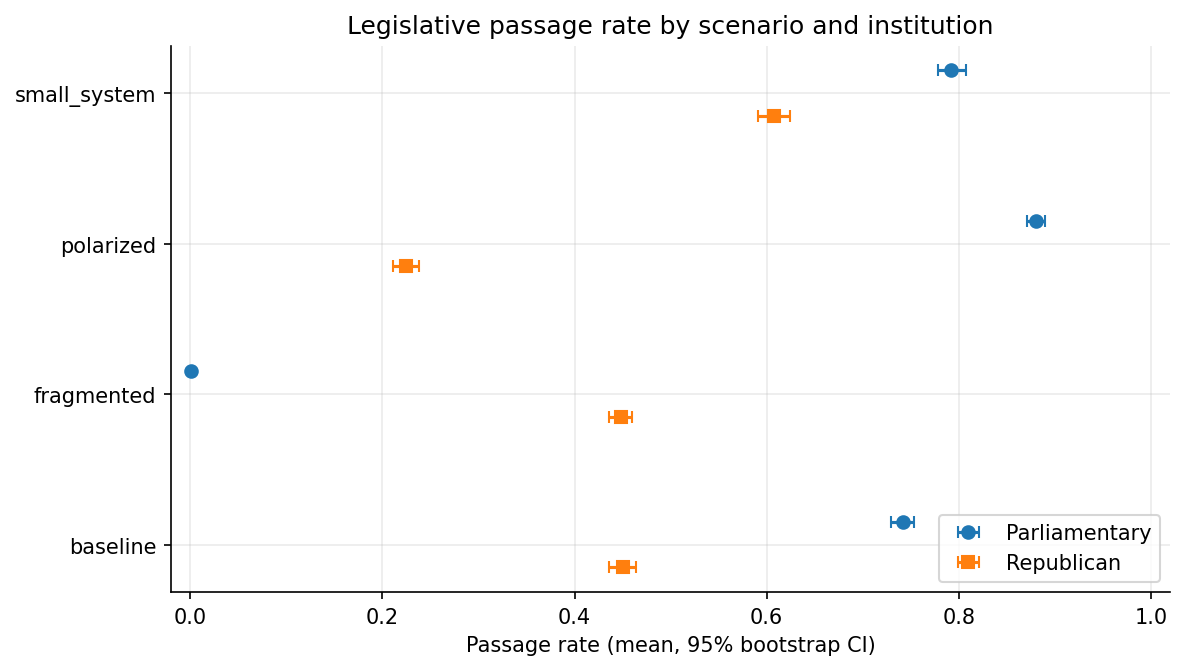
\includegraphics[width=0.98\linewidth]{forest_passage.png}

\vspace{2mm}
\raggedright
\large
\textbf{Baseline:} parliamentary $+29$pp over republican
(Welch $t=38.9$, Cohen $d=2.88$).
\textbf{Fragmented:} parliamentary and premier-presidential collapse;
president-parliamentary partially rescues.
}

\block{Sensitivity: different bottlenecks}{%
\centering
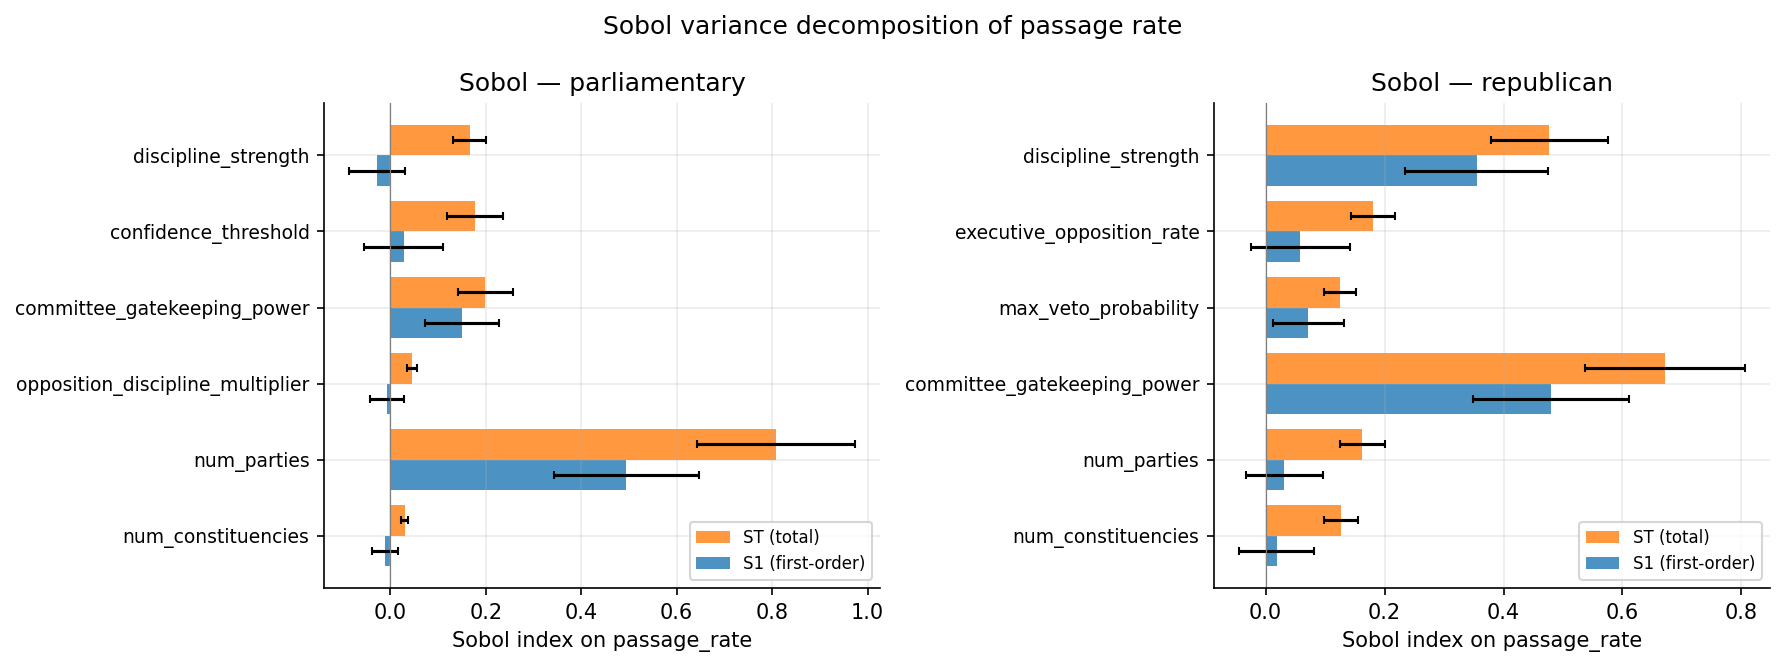
\includegraphics[width=0.98\linewidth]{sobol_bars.png}

\vspace{2mm}
\raggedright
\large
Sobol $S_T$ shows parliamentary passage is dominated by
\texttt{num\_parties} ($0.81$), republican by
\texttt{committee\_gatekeeping} ($0.67$). Structurally different bottlenecks.
}

% ------------------------------------------------------ COLUMN 2 ------------
\column{0.34}

\block{Finding 1a: formation failure is not enough}{%
\centering
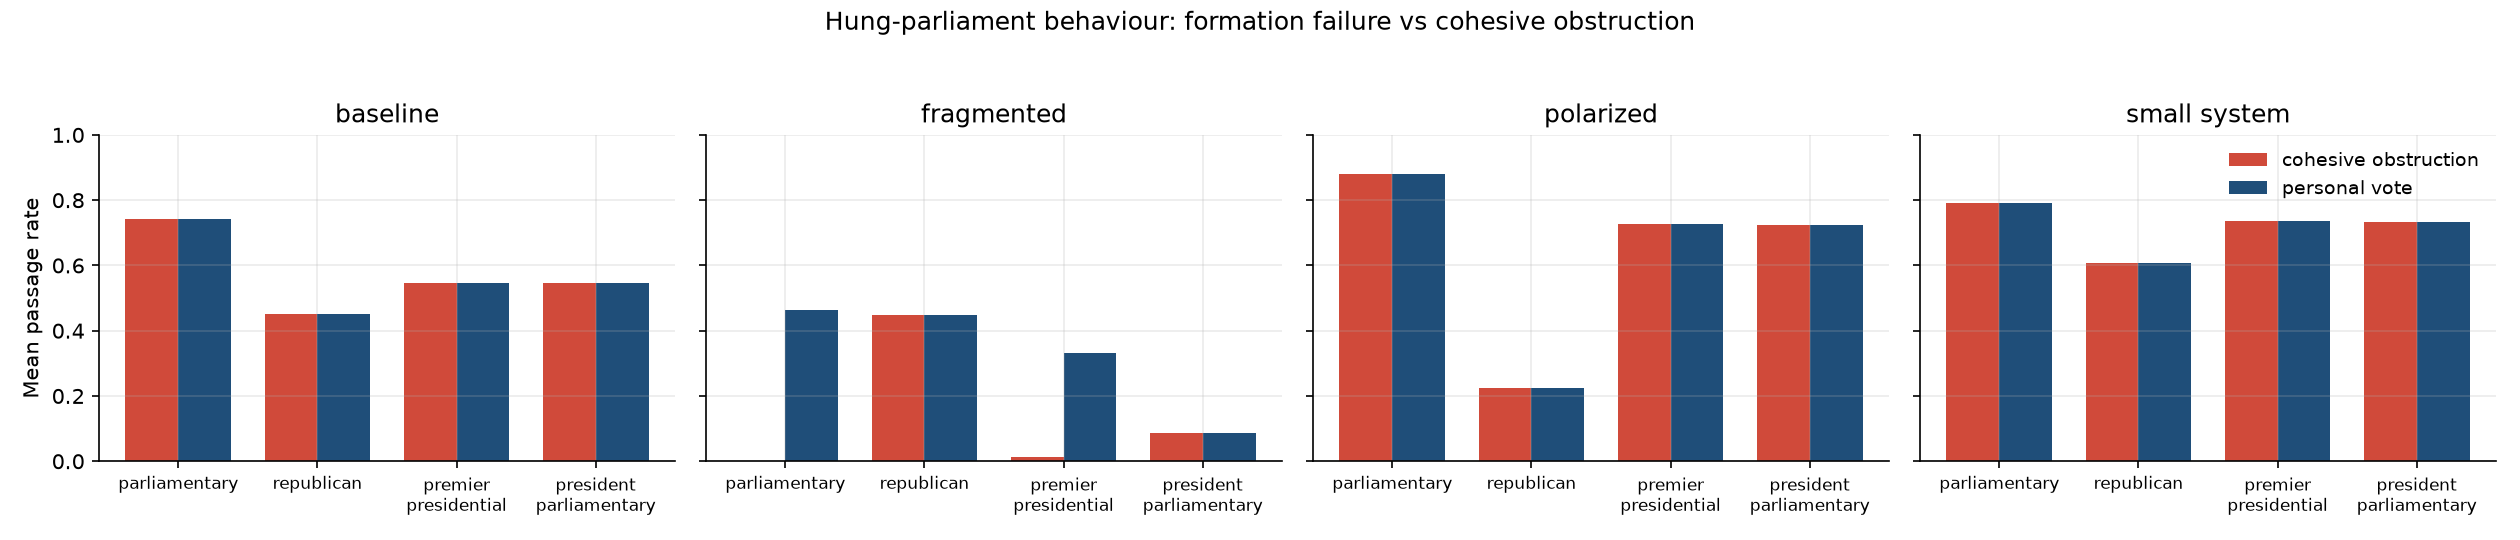
\includegraphics[width=0.98\linewidth]{hung_parliament_comparison.png}

\vspace{2mm}
\raggedright
\large
Fragmentation makes government formation impossible --- but that alone
halts nothing. Letting a hung parliament's MPs vote personally restores
parliamentary passage to $46.4\%$, statistically indistinguishable from
republican's $44.8\%$. Collapse requires \textbf{cohesive opposition
obstruction}: every MP whipped against all business drives passage to
$0.05\%$.
}

\block{Finding 1b: discipline aggregates votes --- both ways}{%
\centering
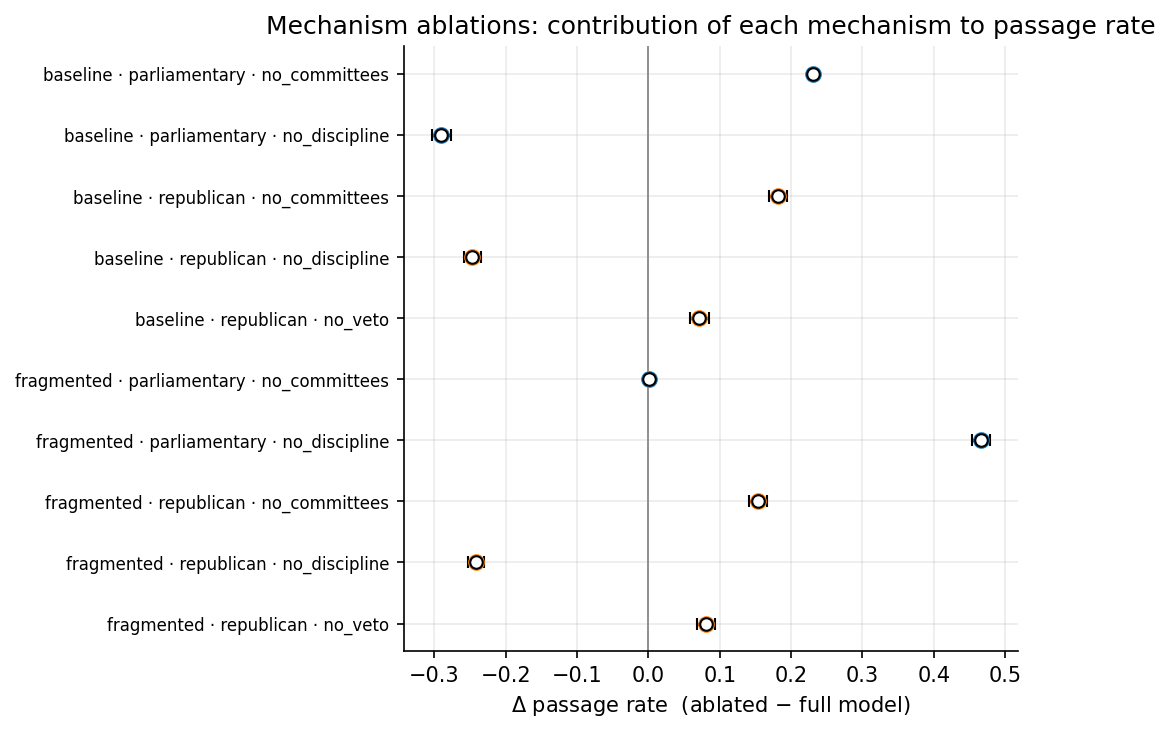
\includegraphics[width=0.98\linewidth]{ablation_forest.png}

\vspace{2mm}
\raggedright
\large
Zeroing the whip (`no\_discipline') restores fragmented parliamentary
passage from $0.05\%$ to $46.7\%$; rescue magnitude falls monotonically
with each institution's dependence on majority government formation.
Under polarisation the same ordering holds with opposite sign:
discipline costs parliamentary $66$pp when bills are extreme. Discipline
aggregates blocs wherever they exist --- governing coalitions pass,
anti-system oppositions obstruct.
}

\block{Finding 2: passage--representation tradeoff}{%
\centering
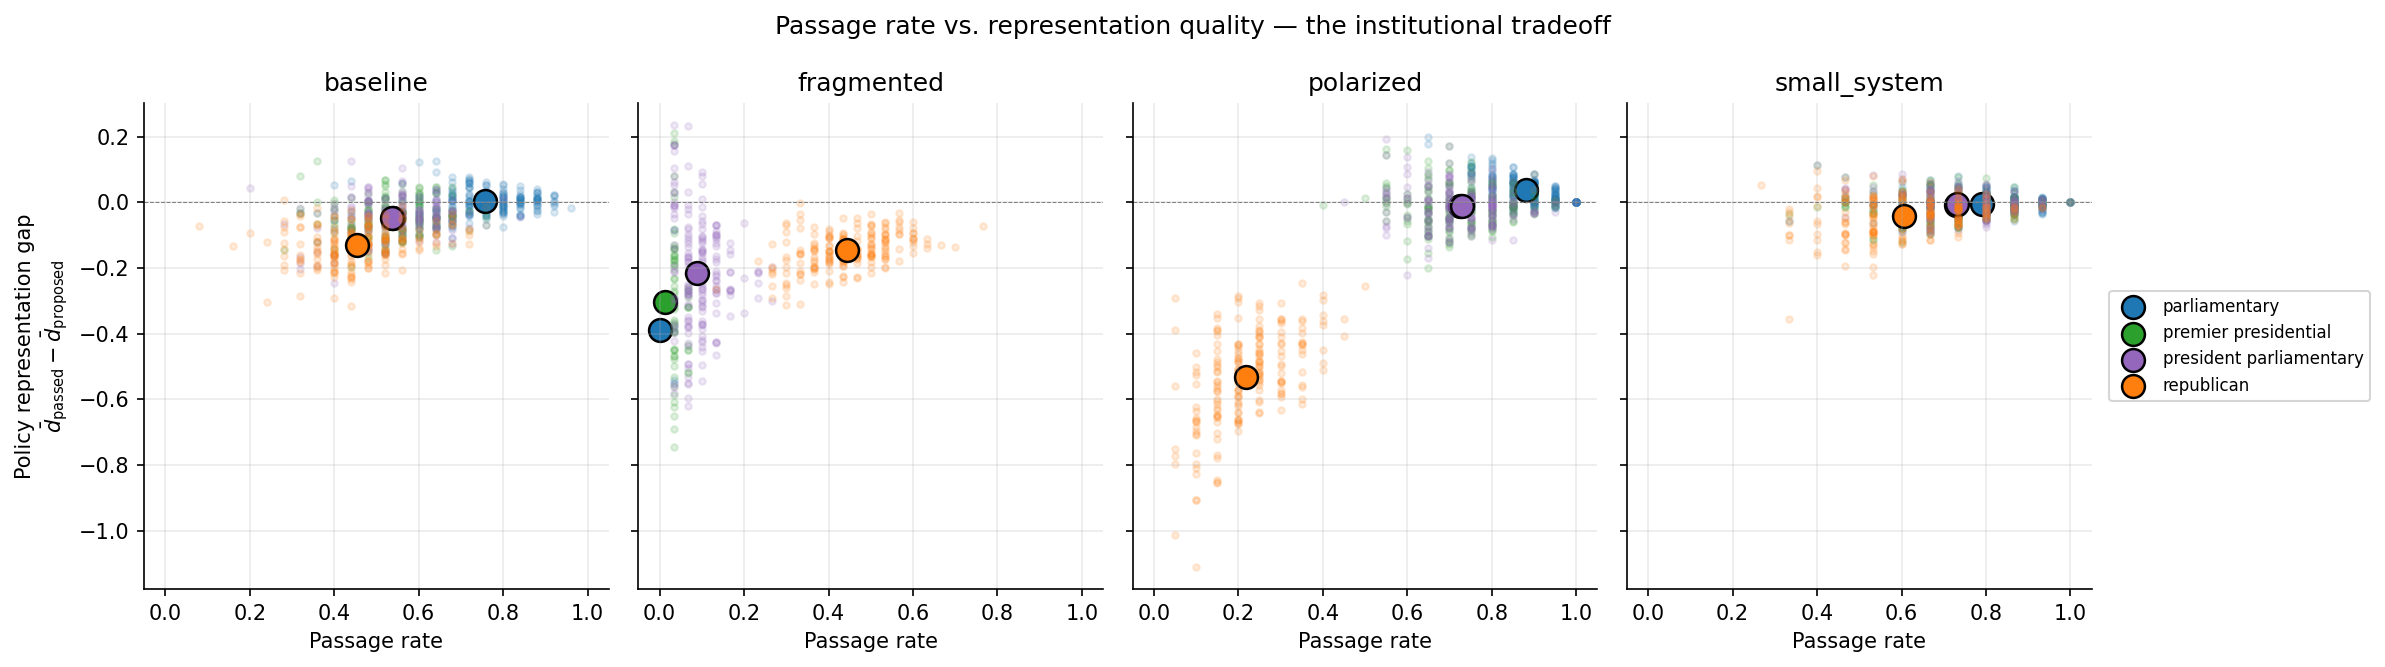
\includegraphics[width=0.98\linewidth]{representation_tradeoff.png}

\vspace{2mm}
\raggedright
\large
Policy representation gap
$= \overline{d_{\text{passed}}} - \overline{d_{\text{proposed}}}$
(L2 distance to constituency median). At polarised:

\vspace{-2mm}
\begin{center}\normalsize
\begin{tabular}{lcc}
\toprule
Institution & Passage & Repr.\ gap \\
\midrule
Parliamentary & $0.882$ & $+0.037$ \\
Premier-pres. & $0.725$ & $-0.012$ \\
President-parl. & $0.730$ & $-0.010$ \\
Republican & $0.218$ & $\mathbf{-0.530}$ \\
\bottomrule
\end{tabular}
\end{center}

\textbf{Filtering and throughput lie on a single spectrum.}
Parliamentary maximises throughput at the cost of filtering; republican
maximises filtering at the cost of throughput; semi-presidential splits.
}

% ------------------------------------------------------ COLUMN 3 ------------
\column{0.33}

\block{Robustness: ordering survives parameter sweeps}{%
\centering
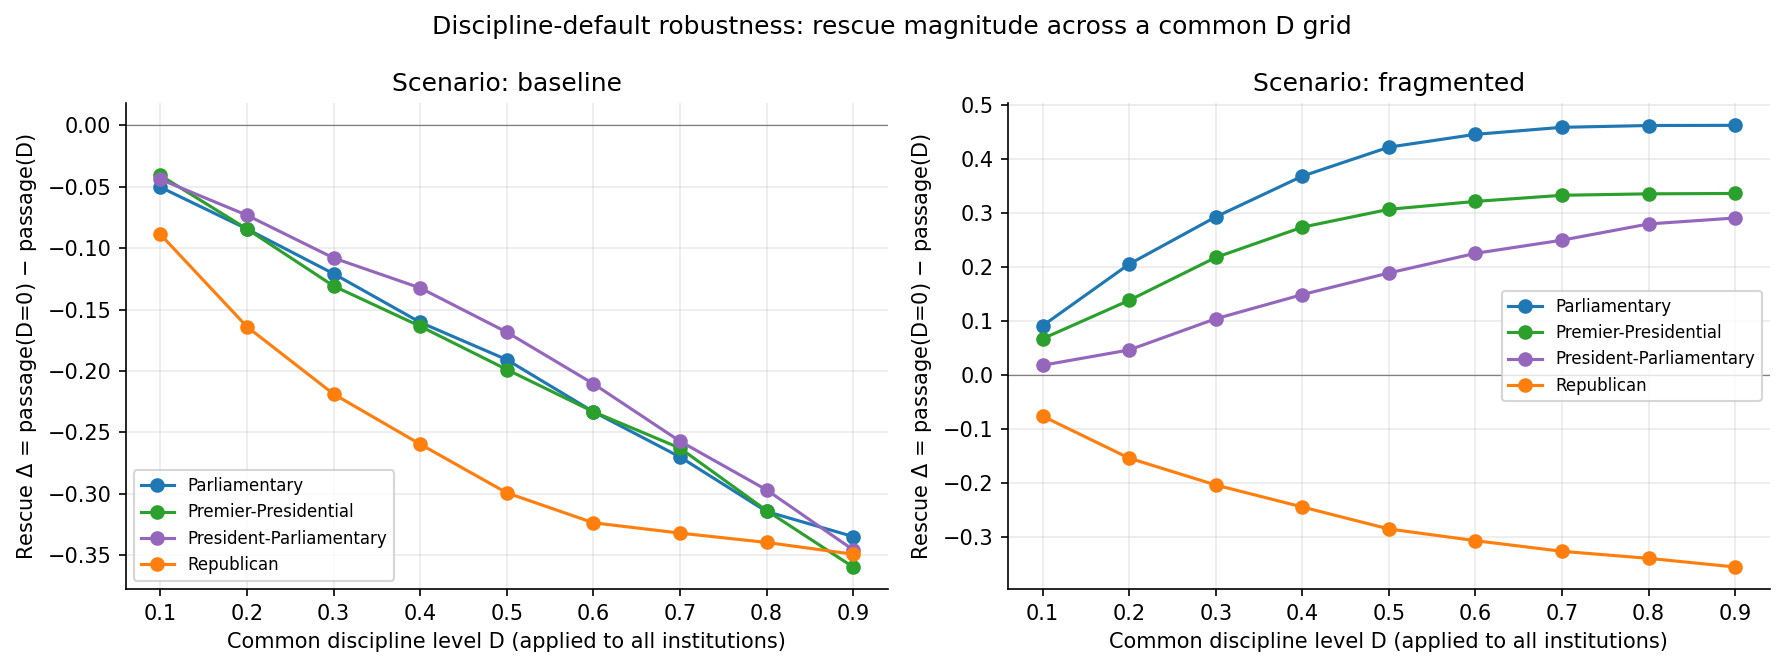
\includegraphics[width=0.98\linewidth]{discipline_rescue_curves.png}

\vspace{2mm}
\raggedright
\large
Set every institution's \texttt{discipline\_strength} to the same $D$
across $\{0.1, \ldots, 0.9\}$. The monotone ordering holds at
\textbf{9/9 tested values under fragmentation}. The structural claim
does not depend on our default parameter choices; a regression test
enforces it.
}

\block{Takeaways}{%
\large
\begin{enumerate}\setlength\itemsep{2.5mm}
    \item \textbf{Coalition failure is not the collapse mechanism.}
        Fragmented parliaments legislate at presidential rates when MPs
        vote personally; cohesive anti-system obstruction is what halts
        them. The pathology lives on the opposition side.
    \item \textbf{Discipline is the universal vote-aggregation mechanism}
        for majority-dependent institutions: it blocks passage under
        obstruction and enables passage under polarisation.
    \item \textbf{The passage--representation tradeoff is one axis.}
        Institutions cannot improve throughput and representational
        fidelity simultaneously; the choice is structural.
    \item \textbf{Reform implication.} Weakening party discipline is an
        alternative to electoral reform for fragmented parliaments ---
        but only where oppositions bargain rather than obstruct.
\end{enumerate}
}

\block{Reproducibility}{%
\large
\begin{itemize}\setlength\itemsep{1.5mm}
    \item Python 3.13, Mesa 2.4, MIT-licensed
    \item $76$ automated tests, GitHub Actions CI
    \item ODD protocol (Grimm et al.\ 2020) in repo
    \item Full paper: \texttt{paper/main.pdf}
    \item Live demo:\\
        \texttt{\small institutional-representation-abm.streamlit.app}
\end{itemize}
}

\block{References}{%
\normalsize
Capoccia (2005).
Cox \& McCubbins (1993).
Laver \& Schofield (1990).
Linz (1990).
Noble \& Schulmann (2018).
Sartori (1976).
Shugart \& Carey (1992).
Str\o m (1984, 1990).
Tsebelis (2002).

\medskip
\small Full bibliography in \texttt{paper/references.bib}.
}

\end{columns}

\end{document}
